\section{Referenční zdroje napětí a proudu}
-jednoduché reference, reference řízené prahovým napětím tranzistoru, bandgap reference, výhody, nevýhody, teplotní závislost, stabilita

\subsection{Jednoduchá reference-napěťové}
Nejjednodušší napěťovou referencí je obyčejný napěťový dělič, ať už s využitím pasivních či aktivních prvků.
\begin{figure}[h]
   \begin{center}
     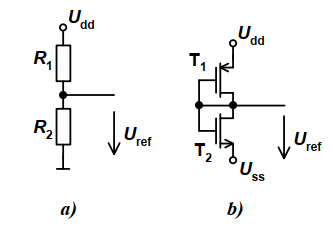
\includegraphics[scale=0.6]{images/ref.png}
   \end{center}
   \caption{Vytvoření napěťové reference pomocí děliče a) rezistorového, b) složeného
z MOST v zapojení jako řízená dioda}
\end{figure}

Velkou nevýhodou zejména zapojení na a) je přímá závislost na napájecím napětí a tedy i přímá závislost na jeho změnách, což lze popsat koeficientem citlivosti S. Zjednodušené řečeno, pokud je S = 1, pak při změně napájecího napětí např. o 10 \% dojde ke stejné změně i na výstupu reference, což je samozřejmě nežádoucí.

Určitého zlepšení lze dosáhnout použitím aktivní součástky (bipolární nebo unipolární tranzistor).
\begin{equation}
 S = \frac{1}{ln\frac{I}{I_{s}}}
\end{equation}
Vzhledem k tomu, že je saturační proud vždy menší jak I, je citlivost menší než jednotková. Např. v případě změny napájecího napětí o 10 \% dojde ke změně reference jen o 0,36 \%.

\begin{figure}[h]
   \begin{center}
     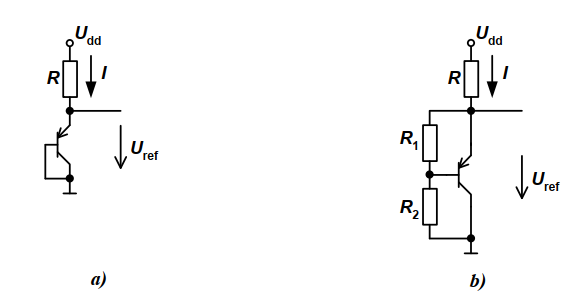
\includegraphics[scale=0.6]{images/ref2.png}
   \end{center}
   \caption{Referenční zdroj s BJT}
\end{figure}
Dalšího zlepšení lze dosáhnout použitím zapojení podle b). Hodnota referenčního napětí je pak:
\begin{equation}
U_{ref} = U_{BE}*(\frac{R_{1}+R_{2}}{R_{1}})
\end{equation}

\pagebreak
Zapojení v kombinaci rezistor s tranzistorem MOS je opět o něco méně závislé na napájení než zapojení s bipolárním tranzistorem. Napětí U\textsubscript{ref} lze odvodit z U\textsubscript{GS}, takže:
\begin{equation}
U_{ref} = U_{GS} = U_{th}+\frac{\sqrt{2*I}}{\beta}
\end{equation}

\begin{figure}[h]
   \begin{center}
     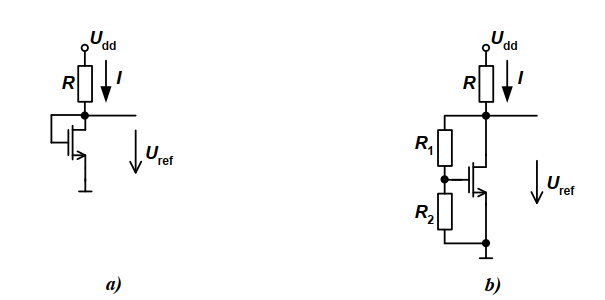
\includegraphics[scale=0.6]{images/ref3.png}
   \end{center}
   \caption{Referenční zdroj s MOS tranzistorem}
\end{figure}

Stejně jako u BJT je výhodnější použití zapojení, jak je uvedeno na b). Referenční napětí je pak:
\begin{equation}
U_{ref} = U_{GS}*(\frac{R_{1}+R_{2}}{R_{1}})
\end{equation}

Velmi přesný referenční zdroj napětí lze realizovat s pomocí silně dopovaného PN přechodu v zapojení v závěrném směru. Jedná se v podstatě o využití průrazného napětí U\textsubscript{br}, buď Zenerova nebo lavinového. Zenerův mechanismus má negativní teplotní koeficient a lavinový má kladný teplotní koeficient.
\begin{figure}[h]
   \begin{center}
     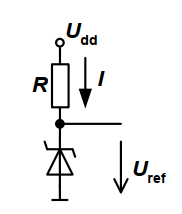
\includegraphics[scale=0.6]{images/refzen.png}
   \end{center}
   \caption{Referenční zdroj se Zenerovou diodou}
\end{figure}

\subsection{Reference řízená prahovým napětím (bootstrapped)-napěťový}
Jestliže je napětí na aktivním prvku (tranzistoru) použito k vytvoření proudu, který je následně využit jako referenční, pak je tento proud nebo napětí na tranzistoru nezávislý na napájecím napětí
\begin{figure}[h]
   \begin{center}
     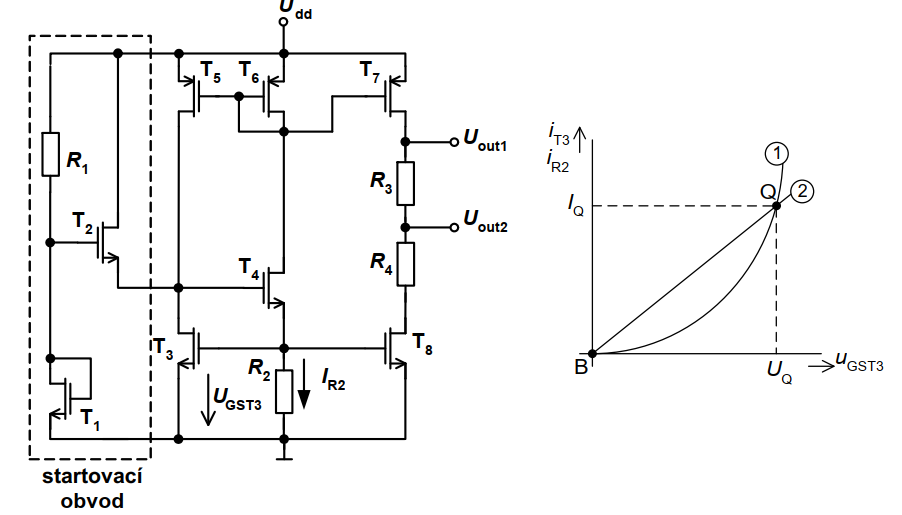
\includegraphics[scale=0.6]{images/BT.png}
   \end{center}
   \caption{Bootstrapped reference a nastavení pracovního bodu}
\end{figure}

Proudové zrcadlo z tranzistorů T\textsubscript{5} a T\textsubscript{6} se stejnými rozměry způsobí, že oběma větvemi teče stejný proud. Proud, který teče tranzistorem T\textsubscript{3} vytvoří úbytek napětí U\textsubscript{GST3}. Zrcadlený proud, který teče přes rezistor R\textsubscript{2}, vytvoří napětí dané jako I\textsubscript{R2} . R2. Vzhledem k tomu, že jsou tato napětí ve společné smyčce, je dosaženo nastavení pracovního bodu.

Aby bylo dosaženo požadovaného referenčního napětí na výstupu, je toto základní zapojení doplněno o tranzistory T\textsubscript{7} a T\textsubscript{8}, čímž se nastavený proud zrcadlí a pomocí odporových děličů jsou nastavena požadovaná referenční napětí.

Problém u tohoto zapojení nastává při nastavování správného pracovního bodu. Obě charakteristiky se vlastně protínají i v bodě B. Tím by ovšem referenční zdroj nepracoval. Aby se tomuto stavu zabránilo, je nutné použít tzv. startovací obvod.

\subsection{Bandgap reference}
Nejpřesnějším a teplotně nejméně závislým referenčním zdrojem je tzv. bandgap reference.
\begin{figure}[h]
   \begin{center}
     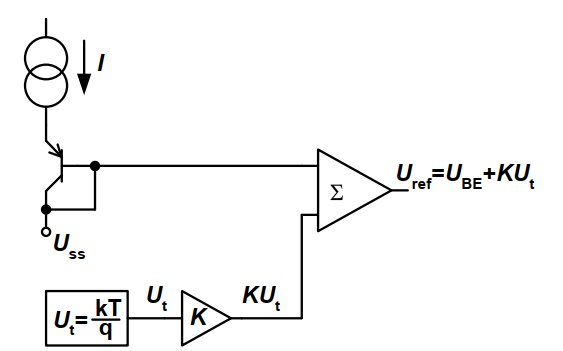
\includegraphics[scale=0.6]{images/BG.png}
   \end{center}
   \caption{Obecný princip bandgap reference}
\end{figure}

Napětí U\textsubscript{BE} je generováno pomocí BJT zapojeného jako dioda, který má nízký teplotní koeficient. Zároveň je generováno teplotní napětí Ut, které je úměrné absolutní teplotě. Pokud je U\textsubscript{t} násobeno konstantou K a připočteno k U\textsubscript{BE} pak je výstupní napětí reference.
\begin{figure}[h]
   \begin{center}
     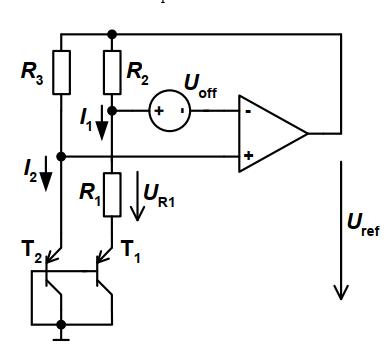
\includegraphics[scale=0.6]{images/BG2.png}
   \end{center}
   \caption{Standardní řešení bandgap reference}
\end{figure}

\begin{equation}
U_{ref} = U_{BE}+K*U_{i}
\end{equation}


\subsubsection{Bandgap reference podle Paula Brokawa}
Pro malé hodnoty napětí V\textsubscript{i} je proud I\textsubscript{1} tranzistorem T\textsubscript{1} větší než proud 
I\textsubscript{2} tranzistorem T\textsubscript{2}, protože T\textsubscript{1} má N-krát větší plochu emitoru. Pro velké proudy je naopak větší proud I\textsubscript{2} tranzistorem T\textsubscript{2}, protože proud I\textsubscript{1} je omezen odporem R. Důležitý je stav ve kterém platí I\textsubscript{1} = I\textsubscript{2}.
Nejpřesnějším a teplotně nejméně závislým referenčním zdrojem je tzv. bandgap reference.
\begin{figure}[h]
   \begin{center}
     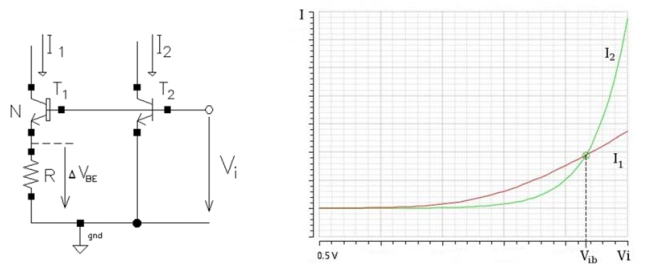
\includegraphics[scale=0.8]{images/Brok.png}
   \end{center}
   \caption{Reference podle P. Brokawa a její průběh}
\end{figure}
\begin{equation}
\Delta U_{BE} = U_{T}*ln(N), I_{1} = I_{2} = I = \frac{U_{T}*ln(N)}{R}
\end{equation}

\subsection{Jednoduchá reference-proudové}
Tyto typy referenčních zdrojů jsou často tvořeny napěťovými referencemi doplněnými pouze o koncový stupeň, který pracuje jako převodník napětí na proud.

Nejjednodušší verzí proudové reference je zapojení, které je tvořeno rezistorem R v zátěži a tranzistory MOS v zapojení jako proudové zrcadlo.
\begin{figure}[h]
   \begin{center}
     \includegraphics[scale=0.6]{images/REFI.png}
   \end{center}
   \caption{Proudový referenční zdroj tvořený proudovým zrcadlem}
\end{figure}

\begin{equation}
I_{ref} = \frac{U_{dd}-U_{GS1}}{R}
\end{equation}

Je zřejmé, že přesnost tohoto typu proudové reference není příliš velká z důvodu silné závislosti na změně napájecího napětí a také z důvodu teplotní závislosti součástek

\subsection{Reference řízená prahovým napětím-proudová}
Reference je založena na napětí úměrnému velikosti prahového napětí tranzistoru, které je přiloženo na daný rezistor

\begin{figure}[h]
   \begin{center}
     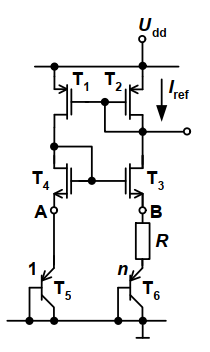
\includegraphics[scale=0.6]{images/PrahI.png}
   \end{center}
   \caption{Proudová reference řízená prahovým napětím tranzistoru}
\end{figure}
\begin{equation}
I_{ref} = \frac{U{T}}{R}*ln(N)
\end{equation}

Pokud budeme uvažovat standardní pokojovou teplotu, pak je teplotní napětí 26 mV a vhodná hodnota N = 8. Napětí na rezistoru je tedy 56 mV, což znamená, že uvedený typ obvodu je vhodný pro generování malých proudů.

\begin{figure}[h]
   \begin{center}
     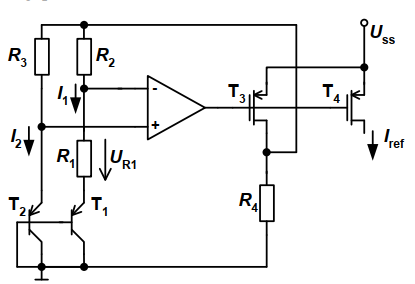
\includegraphics[scale=0.6]{images/PRZ.png}
   \end{center}
   \caption{Proudový referenční zdroj}
\end{figure}


\subsection{Proudový bootstrapped}
Velikost referenčního proudu závisí na napájecím napětí jen velmi málo, protože je v každé větvi vysokoimpedanční prvek (tranzistory T\textsubscript{2} a T\textsubscript{3}), které absorbují případné změny v napájení. Napětí U\textsubscript{ds} tranzistorů T\textsubscript{1} a T\textsubscript{4} se nemůže libovolně měnit, první se pohybuje o dvojnásobek U\textsubscript{gs} nad úrovní země a druhý o U\textsubscript{gs} pod úrovní napájecího napětí. Jakákoli fluktuace napájení je tedy absorbována vysokou rezistencí, která je mezi drainem a sourcem tranzistorů T\textsubscript{2} a T\textsubscript{3}.

\begin{figure}[h]
   \begin{center}
     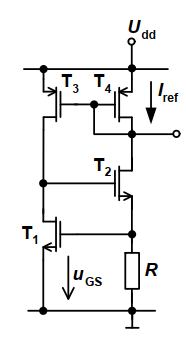
\includegraphics[scale=0.6]{images/BTI.png}
   \end{center}
   \caption{Bootstrapped proudový referenční zdroj}
\end{figure}

Startovací obvod zde není uveden, ale i v tomto případě je nutné jej použít a to ze stejného důvodu jako u napěťové verze, tedy nastavení správného pracovního bodu















\subsection{Výhody a nevýhody}
\textbf{Výhody:} Možnost mít chtěné napětí/proud, které je téměř nezávislé na změnách vstupního napětí

\textbf{Nevýhody:} Jednoduché reference, např. napěťový dělič, jsou velmi nepřesné a citlivé na změnu teploty a napájecího napětí.

\subsection{Teplotní závislost}
Všechny reference jsou samozřejmě více či méně teplotně závislé. Teplotní závislost
reference je definována nejen pomocí koeficientu citlivosti S, ale také pomocí dílčího
teplotního koeficientu (TC\textsubscript{F})
\begin{equation}
TC_{F } = \frac{1}{T}*(S^{X}_T)
\end{equation}
kde X je U\textsubscript{ref} (s použitím převodníku napětí-proud také I\textsubscript{ref}).